%%%%%%%%%%%%%%%%%%%%%%%%%%%%%%%%%%%%%%%%%%%%%%%%%%%%%%%%%%%%%%%%%%%%%%
%
% Documento PRINCIPAL de Pedometria
% Newsletter da Sociedade Brasileira de Ciência do Solo
%
% Número 5, Novembro de 2014
% 
% Language: Latex
% 
%%%%%%%%%%%%%%%%%%%%%%%%%%%%%%%%%%%%%%%%%%%%%%%%%%%%%%%%%%%%%%%%%%%%%%

% PREÂMBULO
\documentclass[a4paper]{report}

% Língua e codificação
\usepackage[brazilian]{babel}
\usepackage[utf8]{inputenc}
\usepackage[T1]{fontenc}
%\usepackage[latin1]{inputenc}
%\DeclareUnicodeCharacter{00A0}{~}

% para boot
\usepackage{amssymb,amsmath}
\usepackage{siunitx}

% Nota: é preciso incluir o pacote amsmath antes do pacote PEDOMETRIAnews
% porque o último redefine o ambiente de equações
\usepackage{PEDOMETRIAnews}
% Citações numéricas, usando sobrescritos, conforme usado em 'Nature'
% Referências para o pacote natbib: http://merkel.zoneo.net/Latex/natbib.php
\usepackage[numbers, super, sort&compress]{natbib}

% Figuras
\usepackage{graphicx}
\usepackage{float}
\usepackage{wrapfig}

% para Sweave
\usepackage{listings}
\usepackage{Sweave}

% cor para verbatim (ambiente para código fonte)
\usepackage{color}
\let\oldv\verbatim
\let\oldendv\endverbatim
\def\verbatim{\par\setbox0\vbox\bgroup\oldv}
\def\endverbatim{\oldendv\egroup\fboxsep0pt \noindent\colorbox[gray]{0.8}{\usebox0}\par}

% definição de \pedometria e \pedometriabf
\newcommand{\pedometria}{\textsc{PedometriA}}
\newcommand{\pedometriabf}{\textsc{\textbf{PedometriA}}}
\newcommand{\pedoartemetria}{\textbf{\sffamily Pedo[Arte]Metria}}
\newcommand{\pergunta}[1]{\vspace*{5mm}\noindent\pedometriabf{} - #1}
\newcommand{\resposta}[2]{\vspace*{5mm}\noindent\textbf{#1} - #2}

% definição de \PedoArteMetria
\newcommand{\PedoArteMetria}[4]{
  \noindent
  \begin{minipage}[t][0.95\textheight][t]{\textwidth}
    \textbf{\sffamily\Huge Pedo[Arte]Metria}\\
    \vspace*{0.5cm}\\
    \begin{figure}[H]
      \includegraphics[width=\textwidth]{#1}
    \end{figure}
    \vspace*{0.5cm}
    \raggedleft
    \begin{minipage}{0.8\textwidth}
      \raggedleft
      \LARGE
      \noindent\textbf{#2}\\
      \vspace*{0.5cm}
      \noindent{#3}
      \vspace*{0.5cm}\\
      \normalsize{\noindent\textit{Foto enviada por: #4}}
    \end{minipage}
    \vfill
    \raggedright
    \begin{minipage}{0.5\textwidth}
      \rule{\textwidth}{1mm}
      \normalsize
      Se você quer compartilhar conosco uma imagem \textbf{\sffamily Pedo[Arte]Métrica} de sua autoria, envie-a para \href{mailto:pedometria.news@gmail.com}{pedometria.news@gmail.com} com resolução de 300 dpi ou com no mínimo 5Mb, preferencialmente em formato PNG.
    \end{minipage}
  \end{minipage}
  }

% doi
\newcommand*{\doi}[1]{[\href{http://dx.doi.org/\detokenize{#1}}{link}]}
  
% para tcltk-update
\usepackage{shortvrb}
%\usepackage{chapterbib}

\sloppy{}

% links
\usepackage{hyperref} % Deve ser o último pacote carregado
\hypersetup{colorlinks=true, citecolor=blue, linkcolor=blue, urlcolor=blue}

% DOCUMENTO
\begin{document}
 
% Edição da newsletter
\volume{5}
\volnumber{5}
\date{Dezembro de 2014}
\titlepage
% \begin{article}
%    \title{Editorial}
\author{por Alessandro Samuel-Rosa}
\maketitle
\begin{wrapfigure}{l}{0.15\textwidth}
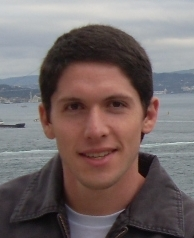
\includegraphics[width=0.15\textwidth]{figuras/foto-alessandro}
\end{wrapfigure}
O segundo número da \textit{Newsletter} da Comissão de Pedometria está cheio de novidades. A principal delas é a nova estrutura, muito mais bonita, graças à inestimável colaboração da comissão editorial do GRASS News, a newsletter do projeto \href{http://grass.osgeo.org/newsletter/}{GRASS}. Após contato com Martin Wegmann \email{wegmann@biozentrum.uni-wuerzburg.de}, editor-chefe do GRASS News, e Dylan Beaudette \email{debeaudette@ucdavis.edu}, administrador da página da web do GRASS News, formos gentilmente autorizados a usar o arquivo de estilo \texttt{GRASSnews.sty}, originalmente derivado do arquivo de estilo \texttt{Rnews.sty}, usado pela equipe do projeto \R{} para produção da sua newsletter. O agora arquivo de estilo da \textit{Newsletter} da Comissão de Pedometria da SBCS, \texttt{PEDOMETRIAnews.sty}, está disponível para baixar \href{http://goo.gl/OBWF3s}{clicando aqui}. É por meio do arquivo de estilo \texttt{PEDOMETRIAnews.sty} que a \textit{Newsletter} fica com a cara que ela tem hoje. Mais informações sobre o uso de \LaTeX{} para a produção de documentos técnico-científicos podem ser encontradas no site da \href{http://www.elsevier.com/author-schemas/preparing-documents-with-tex}{Elsevier}.\\
A evolução da \textit{Newsletter} em seu segundo número acompanha a evolução da pedometria no Brasil, claramente evidenciada pelo volume de trabalhos publicados no Congresso Brasileiro de Ciência do Solo (CBCS), em Florianópolis, há alguns meses atrás. Somam-se aí os espaços destinados mesas de discussão constituídas por importantes pesquisadores da pedometria nacional e internacional. O espaço destinado pela Comissão Organizadora do CBCS mostra que a comunidade científica nacional, assim como já ocorre há mais de uma década em outros países, está muito interessada nas contribuições da mais nova disciplina da ciência do solo. Uma disciplina que exige, como mostram os artigos que seguem, uma abordagem mais do que multidisciplinar ou interdisciplinar. Uma disciplina que exige uma abordagem \href{http://www.fisica-interessante.com/files/artigo-transdisciplinaridade.pdf}{transdisciplinar}, forçando-nos a transpor os limites das disciplinas tradicionais da ciência do solo e mergulhar em um universo de novas maneiras de 
encarar velhos problemas.
%%% Local Variables: 
%%% mode: latex
%%% TeX-master: documento-principal.tex
%%% End: 


% \end{article}
% \newpage
% \PedoArteMetria{fig/}{}{}{}

\newpage
\begin{article}
   \title{Sistema de Informação de Solos Brasileiros}
\author{por Stanley Robson de Medeiros, Humberto Gonçalves dos Santos, e Eliane de Paula Clemente}
\maketitle

\newcommand{\SISB}{\href{http://www.bdsolos.cnptia.embrapa.br/consulta_publica.html}{SISB}}

\subsection{Descrição}

O Sistema de Informação de Solos Brasileiros (\SISB) foi desenvolvido com o objetivo de armazenar, gerenciar, recuperar e disponibilizar informações de perfis de solos brasileiros. O banco de dados reúne atributos de solos coletados e analisados de todas as regiões do Brasil, que podem ser acessados via internet. A partir desta base, aplicações podem ser desenvolvidas para auxiliar a tomada de decisões no agronegócio, classificação de solos, zoneamento agrícola, estimativa da produtividade de solos e subsidiar projetos de ensino e pesquisa. A base de dados será continuamente alimentada por pesquisadores da Embrapa e instituições parceiras.

\subsection{Estrutura hierárquica das informações sobre solos}

A principal característica desse sistema é reunir dados de perfis de solos, análises de fertilidade e mapas (\autoref{fig:estrutura}). Os perfis serão úteis, principalmente, para pesquisadores e estudantes da área de Ciência do Solo. Os módulos sobre fertilidade e mapeamento foram idealizados mas ainda não possuem dados, podendo, no futuro subsidiar a tomada de decisões dos agricultores, além do zoneamento agrícola. As informações georreferenciadas complementarão o banco de dados, fornecendo mecanismos de busca eficientes sobre informações de solos disponíveis no território nacional.

\begin{figure*}[tb!]
  \begin{minipage}[t]{\linewidth}
    \centering
    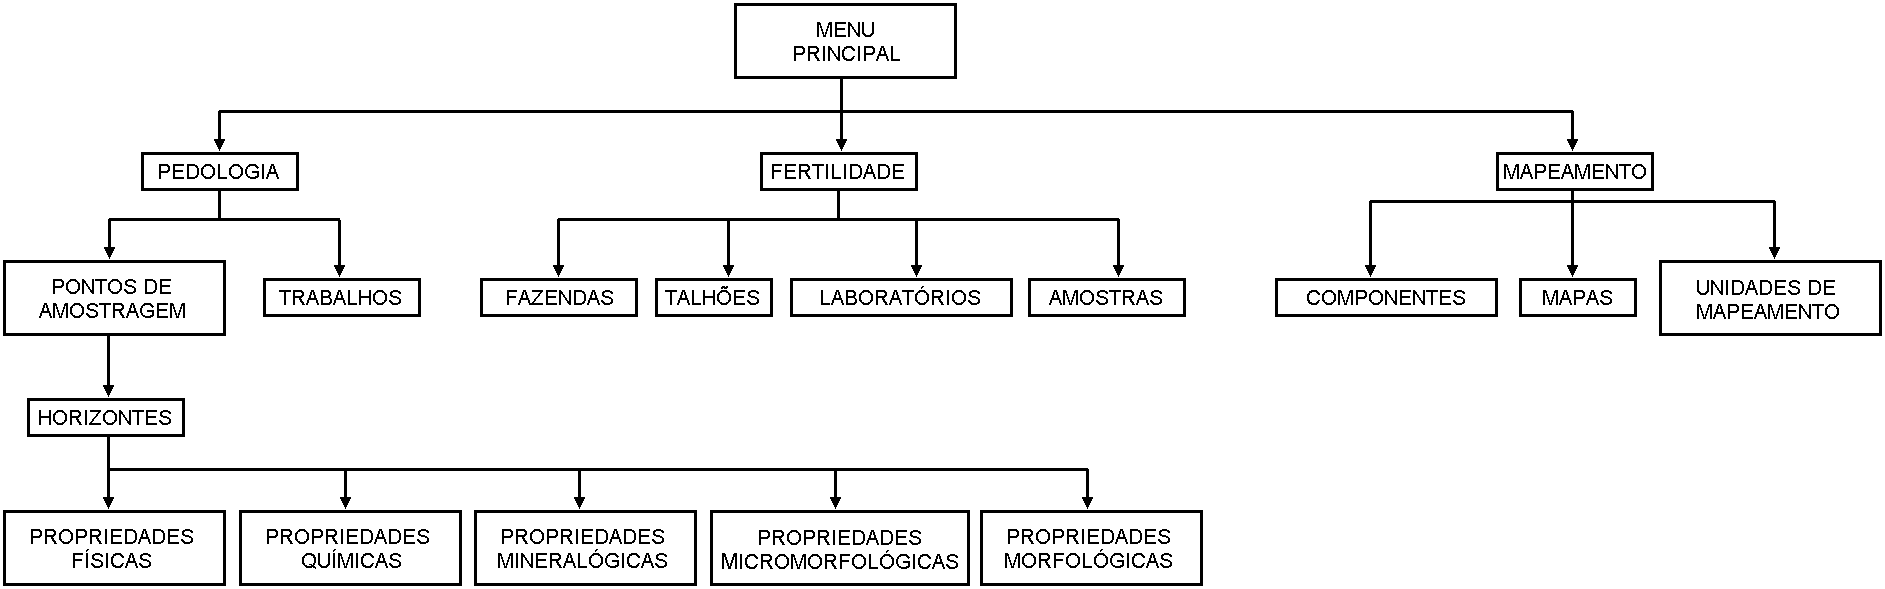
\includegraphics{figuras/estrutura}
    \caption{Estrutura hierárquica do Sistema de Informação de Solos Brasileiros.}
    \label{fig:estrutura}
  \end{minipage}
\end{figure*}

\paragraph{Pedologia} A base de pedologia congrega dados sobre pontos de amostragem (perfis de solos) e é a parte primordial desse sistema de informação. Perfil é a unidade básica de estudo do solo, constituído por seções mais ou menos paralelas à superfície denominadas horizontes ou camadas. Para cada perfil, o sistema armazena informações sobre propriedades físicas, químicas, mineralógicas, morfológicas e micromorfológicas. Informações de física de solos, tais como dados físico - hídricos em geral, densidade do solo, retenção de umidade, micro e macroporosidade, são escassos na base de dados, já que são dados pouco explorados nos levantamentos de solos e nem sempre constituía uma preocupação dos executores de  levantamentos de solos no passado.

\paragraph{Fertilidade} Esta base congrega amostras de solos provenientes de Unidades de Produção Agrícola - UPA - não oriundas de perfis de solos. O módulo de fertilidade foi integrado ao Sistema de Solos com a finalidade de apoiar a tomada de decisões para agricultores.

\paragraph{Mapeamento} Além de mapas, este módulo contém informações sobre Unidades de Mapeamento, que podem ser entendidas como polígonos definidos ou descritos por um critério de relação solo paisagem. Cada Unidade de Mapeamento é composta por um ou mais \textit{Componentes}, que são entidades relativamente homogêneas e identificáveis de uma área, para a qual uma série de valores de propriedades pode ser armazenada. Este módulo de mapeamento não foi completamente desenvolvido e portanto não está disponível no módulo de consulta.

\subsection{Principais benefícios}

Do ponto de vista prático, o sistema será útil para dar suporte à geração de projetos de pesquisa e à tomada de decisões do agronegócio, como, por exemplo, em zoneamento agrícola e em estimativa da produtividade dos solos com base em dados de perfis representativos de classes de solos. No âmbito do ensino e pesquisa, professores, pesquisadores e alunos de pós-graduação podem ser beneficiados com as informações disponíveis no sistema. Além disso, pode-se ressaltar que o uso de dados disponíveis no sistema, serve de base para estudos agronômicos, tais como, mapas de solos, mapas de fertilidade, aptidão agrícola para culturas, zoneamentos climáticos e agroecológicos, dentre outros.

\subsection{Módulo de consultas}

O sistema incorpora amostras e perfis de solos de todo Brasil, apresentando uma descrição detalhada das características morfológicas, físicas, químicas e mineralógicas de perfis representativos, com suas localizações geográficas. Organizadas em um banco de dados único, as informações existentes podem ser facilmente recuperadas, via internet, e utilizadas pelos setores interessados.

\subsection{Sistema Brasileiro de Classificação de Solos – SiBCS}

Os dados armazenados seguem o formato do SiBCS, colaborando para o fortalecimento do sistema de classificação e facilitando a utilização dos dados que estão em formato normatizado e publicado.

\subsection{Parceria}

O Sistema de Informação de Solos Brasileiros é produto da parceria entre a Embrapa Solos e a Embrapa Informática Agropecuária.

\address{Stanley Robson de Medeiros\\
  Embrapa Informática Agropecuária, Campinas, SP\\
  \url{www.embrapa.br/informatica-agropecuaria}\\
  \email{stanley.oliveira@embrapa.br}}

\address{Humberto Gonçalves dos Santos\\
  Embrapa Solos, Rio de Janeiro, RJ\\
  \url{www.embrapa.br/solos}\\
  \email{humberto.santos@embrapa.br}}

\address{Eliane de Paula Clemente\\
  Embrapa Solos, Rio de Janeiro, RJ\\
  \url{www.embrapa.br/solos}\\
  \email{eliane.clemente@embrapa.br}}
%%% Local Variables: 
%%% mode: latex
%%% TeX-master: 5th-edition.tex
%%% End: 
\end{article}

% \newpage
% \begin{article}
%    \input{artigo-giasson}
% \end{article}

\newpage
\begin{article}
   \title{Relatório da Biblioteca Espectral de Solos do Brasil}
\author{por Alexandre Demattê e Alessandro Samuel-Rosa}
\maketitle

\newcommand{\BESB}{\href{http://bibliotecaespectral.wix.com/esalq}{BESB}}
\newcommand{\GeoCIS}{\href{http://esalqgeocis.wix.com/geocis}{GeoCIS}}
\newcommand{\GESB}{\href{https://uspdigital.usp.br/tycho/gruposPesquisaObter?codigoGrupoPesquisa=00675018IPZBKR}{GESB}}

A equipe da Biblioteca Espectral de Solos do Brasil (\BESB) agradece a todos que até o momento puderam colaborar com esta iniciativa única no Brasil. É no mesmo sentido que encorajamos todos a continuar colaborando e a fomentar novas colaborações. Ainda há muito trabalho a ser feito para atingirmos um nível mínimo de representatividade do solo brasileiro.

Neste documento apresentamos um relato das atividades desenvolvidas até agora.

\section{Participantes}

\begin{itemize}
  \item Um total de 18 pesquisadores de 18 instituições de ensino/pesquisa já colaboraram efetivamente com a BESB;
  \item Recebemos um total de \num{2116} amostras de todo o Brasil;
  \item O maior colaborador foi o Grupo de Pesquisa em Geotecnologia em Ciência do Solo (\GeoCIS) que compartilhou \num{162097};
  \item Encerramos o ano de 2014 com um total de \num{19097} amostras;
  \item Já atingimos 17 estados da federação, mas com cobertura variada. Os estados são: Rio Grande do Sul, Santa Catarina, Paraná, São Paulo, Mato Grosso do Sul, Mato Grosso, Rio de Janeiro, Bahia, Pernambuco, Maranhão, Amazonas, Acre, Paraíba, Rio Grande do Norte, Pará, Ceará, Roraima, e Alagoas;
  \item Já temos os dados espectrais de todas estas amostras com uma análise global já implementada. Explicamos \SI{75}{\percent} da variância da argila mesmo sem nenhum tratamento dos dados.
\end{itemize}

\begin{figure}
  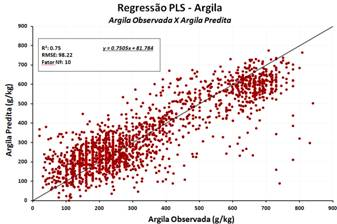
\includegraphics{figuras/image003}
\end{figure}

\section{Tipos de amostras}

Vários tipos de amostras foram recebidas durante o ano de 2014, a saber:

\begin{itemize}
  \item Amostras simples;
  \item Amostras em profundidade coletada com trado;
  \item Amostras de horizontes de perfis completos.
\end{itemize}

O recebimento de amostras variadas foi efetuado nesta etapa para avaliarmos as dificuldades na implementação do projeto.

\section{Métodos}

As amostras recebidas são catalogadas e uma alíquota é armazenada, recebendo uma sigla e a identificação do responsável pela amostra. Todos os procedimentos analíticos são realizados usando o sensor Fieldspec. Os dados espectrais são identificados com a mesma sigla da amostra, armazenados no banco de dados, e em seguida ligados ao arquivo MS Office Excel contendo os dados analíticos.

\section{Visitas}

Temos recebido pessoas de fora para visitar o laboratório ou mesmo acompanhar as leituras da própria amostra.

\section{Divulgação na Internet}

As atividades são divulgadas no site da \BESB{} e do Grupo de Pesquisa em Geotecnologia em Ciência do Solo (\GeoCIS) da ESALQ que dá apoio às atividades da BESB.

\begin{figure*}[tb!]
\begin{minipage}[t]{1\linewidth}
   \centering
   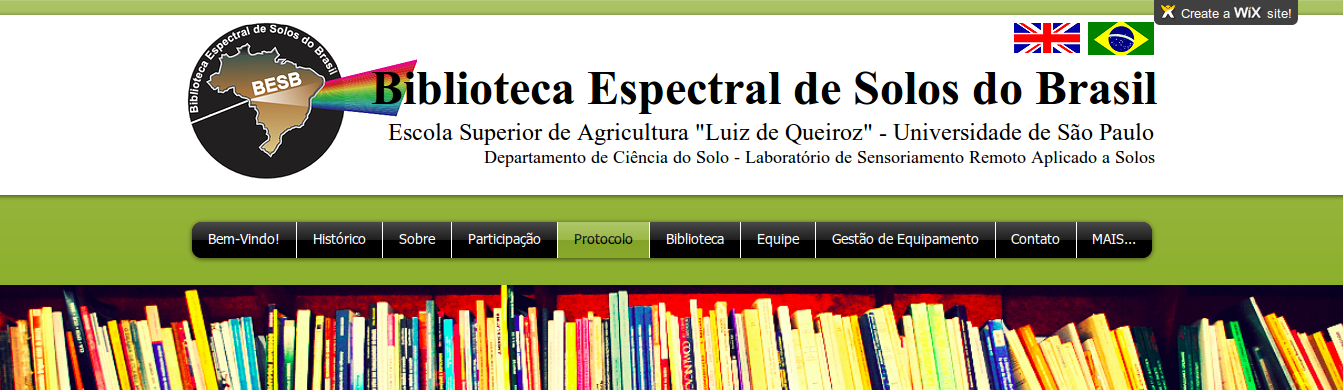
\includegraphics{figuras/image008}
   \caption{Banner da Biblioteca Espectral de Solos do Brasil.}
   \label{fig:banner}
\end{minipage}
\end{figure*}

\begin{figure}
  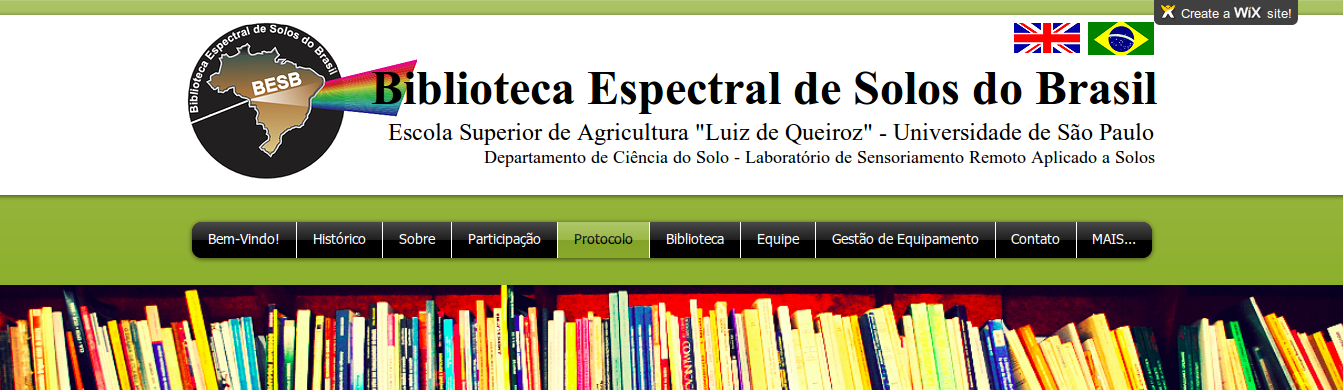
\includegraphics{figuras/image008}
\end{figure}

\section{Divulgação geral}

As BESB já foi divulgada em diversas oportunidades. São elas:

\begin{itemize}
  \item Reunião da FAO em Roma, Itália, em dezembro de 2013;
  \item Davis, Califórnia, EUA, em janeiro de 2014;
  \item College Station, Texas, EUA, em fevereiro de 2014;
  \item Simpósio de Iniciação Cientifica da USP, em dezembro de 2014;
  \item Programa Band Rural, em 2014;
  \item Revista FAPESP;
  \item E aqui na \pedometria.
\end{itemize}

\section{Grupo de pesquisa}

Foi criado o Grupo de Espectroscopia de Solos do Brasil (\GESB). O grupo se encontra em fase de análise no CNPq.

\section{Publicação}

A primeira publicação somente virá após o término do mestrado do aluno que esta fazendo o trabalho. Isto se dará em maio de 2015. Vai tratar desta primeira versão. Logo em seguida segue um novo aluno para partir para a nova e última etapa a seguir descrita. Também será publicado um relatório no formato de Atlas de Solos do Brasil contendo fotos e espectros.

\section{Apresentação e publicação do material}

O material será apresentado no Congresso Brasileiro de Ciência do Solo (CBCS) a ser realizado em Natal em agosto 2015, após o qual será submetido a publicação um artigo de caráter geral. Nele TODOS os colaboradores serão incluídos como co-autores. Esta será o que chamo de primeira versão. pois haverá uma segunda versão hum ano depois, finalizando a etapa de publicações gerais.
Se tudo correr bem, haverá uma palestra sobre o trabalho no CBCS.

\section{Próximas etapas}

O RECEBIMENTO DE AMOSTRAS CONTINUA!!! Mas a partir de agora somente serão aceitas:

\begin{itemize}
  \item amostras de perfis completos, OU
  \item amostras de tradagens completas em profundidade
\end{itemize}

As amostras DEVEM vir acompanhadas de foto do perfil e dados analíticos mínimos:

\begin{itemize}
  \item Granulometria;
  \item Química tradicional;
  \item Classificação taxonômica até o máximo nível categórico possível.
\end{itemize}

O georreferenciamento, apesar de desejado, não é obrigatório, sendo suficiente indicar apenas o município mais próximo. O protocolo para a coleta de perfis completos e uma planilha modelo para envio dos dados estão disponíveis no site da BESB (\href{http://bibliotecaespectral.wix.com/esalq#!protocolo/c1sc5}{acesse aqui}). 

\section{Forma de apresentação}

A \autoref{fig:curvas} mostra o que desejamos atingir na próxima etapa de desenvolvimento da BESB. Na primeira etapa 1, que ora finaliza, conseguimos avançar em direção a este objetivo. Mas a segunda etapa será mais restritiva, exigindo mais as análises e descrição do local e do perfil.

\begin{figure*}[tb!]
\begin{minipage}[t]{1\linewidth}
   \centering
   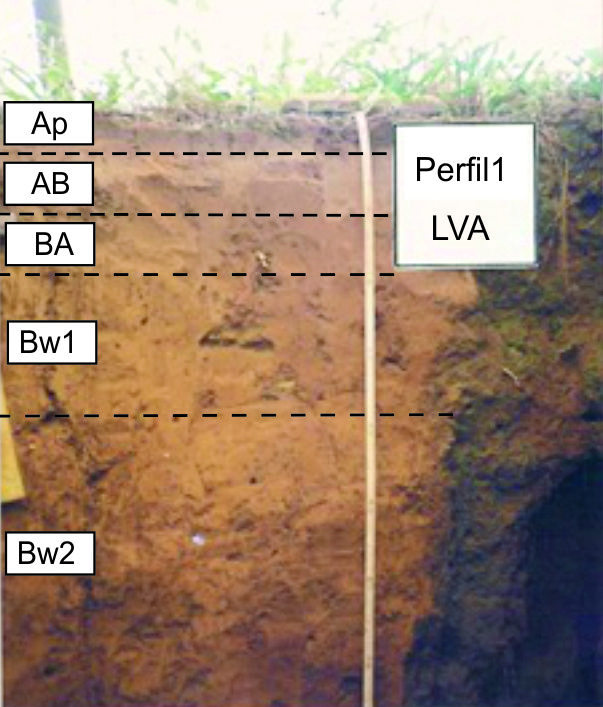
\includegraphics[width=0.49\textwidth]{figuras/lva.jpg}
   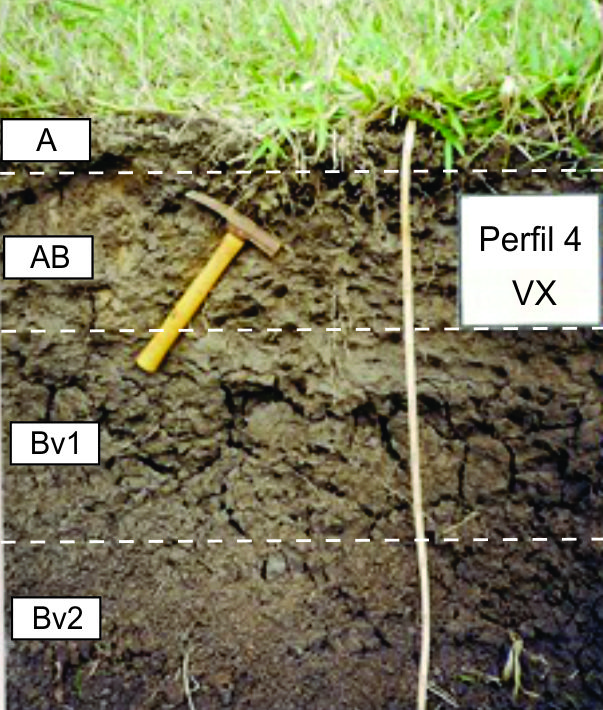
\includegraphics[width=0.49\textwidth]{figuras/vertissolo.jpg}
   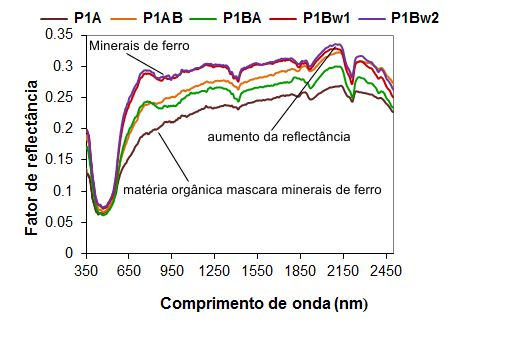
\includegraphics[width=0.49\textwidth, trim=0.5cm 0cm 1.5cm 0cm, clip]{figuras/curvas-lva.jpg}
   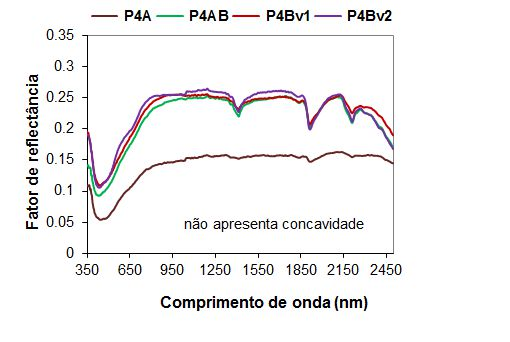
\includegraphics[width=0.49\textwidth, trim=0.5cm 0cm 1.5cm 0cm, clip]{figuras/curvas-vertissolo.jpg}
   \caption{Curvas espectrais dos horizontes de perfis estudados. Solo 1 -- Latossolo Vermelho-Amarelo com horizontes Ap, AB, BA, Bw1, Bw2. Solo 2 -- Vertissolo Háplico com horizontes A, E, Bv1 e Bv2.}
   \label{fig:curvas}
\end{minipage}
\end{figure*}

\section{Dúvidas frequentes}

A maior dúvida dos colaboradores é quanto aos direitos retidos sobre os dados. Muitos parecem ter dificuldade em compartilhar dados devido ao receio de não receber qualquer crédito autoral.

Queremos deixar claro que os dados enviados são de propriedade daquele que os enviou. A equipe da BESB apenas obtém os dados espectrais, e sim, publicaremos um primeiro trabalho, para preservar o nosso trabalho inicial. MAS é um trabalho MACRO, não regional, logo, o ‘dono’ dos dados poderá publicar artigos com os seus dados em caráter regional.

Além disso, os dados ficarão guardados aqui na ESALQ (onde nem eu nem ninguém poderá utiliza-los) e será enviado aos respectivos donos. Este método, permitirá que todos no Brasil, indo no site, saibam QUEM tem dados, e com isso, possam se contatar mutuamente para fazer trabalhos em conjunto fortalecendo a comunidade e aumentando os índices de publicação. De nossa parte o ganho será a citação do trabalho base (Mas com todos co-autores), o global, a citação da BESB e um atlas.

ESTOU TENDO CERTA DIFICULDADE EM CONVENCER ALGUNS COLEGAS. PRECISAMOS DE PERFIS COMPLETOS A PARTIR DE AGORA COM FOTOS. ISSO VAI GERAR UM ATLAS DE IMPACTO IMPORTANTE E FICAR POR GERAÇÕES. PECO A TODOS OS  QUE VEREM ESTE MAIL, REPASSEM A COLEGAS PEDÓLOGOS, SENSIBILIZANDO-OS AO CUSTO/BENEFICIO DESTA INICIATIVA. A PARTICIPAÇÃO DEVE SER DE PEDÓLOGOS QUE TEM ACERVOS OU AMOSTAS DE PERFIS COMPLETOS COM FOTOS E DESCRIÇÕES.

Vejam, o pedólogo não vai perder estes dados NEM que ele mesmo pense em  gerar artigos em espectroscopia, pois o que vira para nos será usado para um atlas e para uma publicação de caráter geral. Estas duas publicações NÃO inviabilizam publicações regionais, aprofundadas com os dados. Ademais, tem pedólogos que estão guardando material que nem sabem se um dia irão usar para espectroscopia! Com isso, o BRASIL vai ficar sem estes dados a disposição da comunidade. Mostrar um espectro num atlas não inviabiliza a publicação do processamento e estudo do mesmo! Ademais, no ATLAS, os nomes dos doadores estarão sendo divulgados!
 
Esta iniciativa é para deixar algo para o futuro do pais, para os novos pedólogos e gerações.
 
Continuo a disposição para esclarecimentos.
O projeto continua!
Abcs


19-34172109
 
QUEM ACREDITAR NA INICIATIVA, POR FAVOR REPASSEM AO MAIOR NUMERO DE COLEGAS PDOLOGOS POSSIVEL!!!! E QUE ENTREM EM CONTATO COMIGO!

\address{Alexandre Demattê\\
  Departamento de Ciência do Solo, ESALQ/USP\\
  \url{http://www.solos.esalq.usp.br/docentes.htm}\\
  \email{jamdemat@usp.br}}

\address{Alessandro Samuel-Rosa\\
  ISRIC - World Soil Information\\
  \url{http://www.soil-scientist.net}\\
  \email{alessandro.rosa@wur.nl}}
%%% Local Variables: 
%%% mode: latex
%%% TeX-master: 5th-edition.tex
%%% End: 
\end{article}

\newpage
\begin{article}
   \title{Eventos}
\maketitle


\section{INTERGEO}
\subsection{Istambul, Turquia, 28-29/4/2014}
O congresso é organizado pela German Society of Geodesy, Geoinformation and Land Management (DVW). 
Maiores informações podem ser encontradas no endereço \url{http://www.intergeo-eurasia.net/en/index.html}.


\section{Conferência e Feira de Geomática e Soluções Geoespaciais}
\subsection{São Paulo, Brasil, 7-9/5/2014}
O evento é organizado por MundoGEO.
Maiores informações podem ser encontradas no endereço \url{http://mundogeoconnect.com/2014/}.


\section{ISRIC'S Spring School 2014}
\subsection{Wageningen, Holanda, 12-16/5/2014}
O evento é organizado pelo International Soil Reference and Information Centre - ISRIC. Serão abordados temas relacionados ao Mapeamento Digital de Solos (MDS) e uso de softwares para análise de dados de solos.
Maiores informações podem ser encontradas no endereço \url{http://www.isric.org/content/isrics-spring-school-2014}.


\section{20th Word Congress of Soil Science}
\subsection{Jeju, Korea, 8-13/06/2014}
O congresso é organizado pela International Union of Soil Sciences (IUSS). 
Maiores informações podem ser encontradas no endereço \url{http://www.20wcss.org/}.


\section{12th International Conference of Precision Agriculture}
\subsection{Sacramento, Califórnia (USA), 20-23/07/2014}
O congresso é organizado pela Sociedade Internacional de Agricultura de Precisão.
Maiores informações podem ser encontradas no endereço \url{https://www.ispag.org/ICPA/}.


\section{XX Congresso Latinoamericano de la Ciencia Del Suelo}
\subsection{Cusco, Perú, 9-15/11/2014}
O evento é organizado pela Sociedade Latinoamericana de Ciência do Solo (SLCS).
Maiores informações podem ser encontradas no endereço \url{http://www.xxcongresolatinoamericanodesuelosperu.org/programa.php}.


\section{6th Global Workshop on Digital Soil Mapping}
\subsection{Nanjing, China, 11-14/11/2014}
O evento é  organizado pelo Instituto de Ciência do Solo da Academia Chinesa de Ciências. O prazo para submissão de trabalhos é 31/07/2014.
Maiores inforamçoes podem ser encontradas no endereço \url{http://dsm2014.csp.escience.cn/}.


\address{Jean Michel Moura-Bueno\\
    Universidade Federal de Santa Maria\\
    \email{bueno.jean1@gmail.com}}
\end{article}

\newpage
\begin{article}
   \title{Pedometria na SBCS}
\maketitle
\newcommand{\estrutura}{\href{http://www.sbcs.org.br/a-sbcs/estatuto/}{estrutura científica}}
\newcommand{\SBCS}{\href{http://www.sbcs.org.br/}{SBCS}}
\newcommand{\IUSS}{\href{http://www.iuss.org/}{IUSS}}
\newcommand{\boletim}{\href{http://www.iuss.org/images/stories/IUSS\%20Bulletin\%201\%20-\%20117/00000097.pdf}{Boletim 97}}
\newcommand{\EspacoTempo}{\href{http://www.sbcs.org.br/comissoes-especializadas/divisao-1-solo-no-espaco-e-no-tempo/}{Espaço e no Tempo}}
\newcommand{\PedometronOnze}{\href{http://www.pedometrics.org/Pedometron/pedometron11.pdf}{Pedometron 11}}
\newcommand{\PedometronDoze}{\href{http://www.pedometrics.org/Pedometron/pedometron12.pdf}{Pedometron 12}}

A atual \estrutura{} da Sociedade Brasileira de Ciência do Solo (\SBCS) foi definida na Assembleia Geral dos Congressos Brasileiros de Ciência do Solo realizados em Fortaleza (2009) e Uberlândia (2011). Na época, o objetivo principal foi adequar-se a estrutura científica da União Internacional de Ciência do Solo (\IUSS), a qual fora definida no Congresso Mundial de Ciência do Solo realizado na Tailândia em 2002. Tal estrutura inclui Divisões, Comissões, Grupos de Trabalho, e Comitês Permanentes (\boletim). São as Divisões, as Comissões e os Grupos de Trabalho os responsáveis por desenvolver as atividades científicas da SBCS e da IUSS.

Hoje são quatro as Divisões da SBCS e da IUSS, cada uma subdividida em Comissões. A Divisão I da SBCS, chamada Solo no \EspacoTempo, possui três Comissões: Gênese e Morfologia do Solo, Levantamento e Classificação do Solo, e Pedometria.

A coordenação da Divisão I é a seguinte:

\begin{itemize}
 \item Diretor: Lúcia Helena Cunha dos Anjos - UFRRJ
 \item Vice-diretor: Humberto Gonçalves dos Santos - EMBRAPA
 \item Membro titular: Elpídio Inácio Fernandes Filho - UFV
 \item Membro suplente: Cristiane Valéria de Oliveira - UFMG
\end{itemize}

\subsection{Comissão de Pedometria}

A Comissão de Pedometria da IUSS foi criada no Congresso Mundial de Ciência do Solo realizado na Tailândia em 2002 a partir do Grupo de Trabalho em Pedometria, um dos mais ativos na época. Muitas foram as discussões sobre a Divisão a qual a Comissão de Pedometria deveria pertencer (\PedometronOnze{} e \PedometronDoze). Isso porque a pedometria constitui um campo que abrange muitos outros campos da ciência do solo, como estatística, matemática, física, química, informática, biologia, mineralogia, geografia \textit{et cetera}. Apesar da multitude de campos de atuação, a nova estrutura científica da IUSS exige que as Comissões façam parte de uma única Divisão. Como a maior parte das contribuições da pedometria estão relacionadas à variabilidade espaço-temporal das propriedades do solo, o consenso foi de que a Divisão I seria a mais apropriada.

A Comissão de Pedometria da SBCS possui em seu escopo os seguintes temas:

\begin{itemize}
 \item Fotointerpretação e sensoriamento remoto
 \item Mapeamento digital de solos
 \item Variabilidade espacial e temporal de atributos de solo (geoestatítica)
 \item Análise espectral (refletância)
 \item Processamento de dados de solos
\end{itemize}

A coordenação da Comissão de Pedometria é a seguinte:

\begin{itemize}
 \item Coordenador: Maria de Lourdes Mendonça Santos - EMBRAPA
 \item Vice-coordenador: Elpídio Inácio Fernandes Filho - UFV
 \item Membros titulares: César da Silva Chagas - EMBRAPA, e José Alexandre Melo Demattê - ESALQ/USP
 \item Membros suplentes: Gustavo de Mattos Vasques - EMBRAPA, e Ricardo Simão Diniz Dalmolin - UFSM
\end{itemize}

\subsection{Grupo de Trabalho em Mapeamento Digital de Solos}

Os Grupos de Trabalho são grupos científicos criados em caráter temporário para tratar de problemas específicos da ciência do solo. Atualmente a IUSS possui 17 Grupos de Trabalho atuando nos mais diversos temas.

O primeiro Grupo de Trabalho da SBCS foi criado durante o Congresso Brasileiro de Ciência do Solo realizado em Florianópolis (2013). Trata-se do Grupo de Trabalho em Mapeamento Digital de Solos (GT-MDS). A solicitação foi feita pela Rede Brasileira de Pesquisa em Mapeamento Digital de Solos (RedeMDS), constituída por pesquisadores de diversas instituições de ensino e pesquisa brasileiras.

O GT-MDS possui como missão elaborar projetos de ação conjunta e integrada para o mapeamento digital dos solos do Brasil e gerar sinergia entre os pesquisadores brasileiros para promover o avanço da pesquisa em mapeamento digital de solos.

Especificamente, o GT-MDS possui como objetivos:

\begin{itemize}
 \item Consolidar a Rede Brasileira de Mapeamento Digital de Solos do Brasil
 \item Realizar o mapeamento digital de atributos do solo em todo o território brasileiro
 \item Realizar o mapeamento digital de classes de solos
 \item Propor metodologia e validação de mapeamento digital de classes e/ou atributos de solos em áreas pilotos do território brasileiro
 \item Realizar treinamento em mapeamento digital de solos
\end{itemize}

A fim de cumprir sua missão e alcançar seus objetivos, o GT-MDS procura realizar encontros anuais. Estes encontros geralmente ocorrem concomitantes a outros eventos de abrangência nacional a fim de estimular a interdisciplinaridade e otimizar os recursos disponíveis. Nos anos em que é realizado o Congresso Brasileiro de Ciência do Solo, o GT-MDS reúne-se para avaliar as atividades científicas passadas, definir as atividades científicas futuras, e faz um relato das mesmas ao Coordenador Geral da Divisão I.

A coordenação atual do GT-MDS é composta pelos seguintes pesquisadores:

\begin{itemize}
 \item Coordenador geral: Márcio Francelino - UFV
 \item Coordenador Regional I: Ricardo Simão Diniz Dalmolin - UFSM
 \item Coordenador Regional II: José Alexandre M. Demattê - ESALQ/USP
 \item Coordenador Regional III: Elpidio Inácio Fernandes Filho - UFV
 \item Coordenador Regional IV: Gustavo de Mattos Vasques - EMBRAPA SOLOS
 \item Coordenador Regional V: Gustavo Souza Valladares - UFPI
\end{itemize}
%%% Local Variables: 
%%% mode: latex
%%% TeX-master: 5th-edition.tex
%%% End:
\end{article}

\newpage
\begin{article}
   \title{Instruções aos autores}
\maketitle
\newcommand{\SBCS}{\href{http://www.sbcs.org.br/}{SBCS}}
\newcommand{\Nature}{\href{http://www.nature.com/nature/authors/gta/}{Nature}}
\newcommand{\Science}{\href{http://www.sciencemag.org/about/authors}{Science}}
\newcommand{\CreativeCommons}{\href{http://creativecommons.org/licenses/by-sa/2.0/}{CC-BY-SA}}
\newcommand{\Kile}{\href{http://kile.sourceforge.net/}{Kile}}
\newcommand{\MiKTeX}{\href{http://miktex.org/}{MiKTeX}}
\newcommand{\aquiLaTeX}{\href{https://docs.google.com/document/d/1F3IXzWNCeUrwKeFxA4iHS3aw1nforK1IqB126xbawvA/edit?usp=sharing}{aqui}}
\newcommand{\aquiWord}{\href{https://docs.google.com/document/d/1pyK03RBDPhOMrTVfvj9NcEfjGWeswqYbYDqEKq83drQ/edit?usp=sharing}{aqui}}
\newcommand{\Geoderma}{\href{http://www.elsevier.com/author-schemas/latex-instructions}{Geoderma}}
\newcommand{\EJSS}{\href{http://onlinelibrary.wiley.com/journal/10.1111/\%28ISSN\%291365-2389/homepage/ForAuthors.html}{European Journal of Soil Science}}

\subsection{Escopo e política}

\pedometria{} é a \textit{Newsletter} (boletim técnico-científico) da Comissão de Pedometria da Sociedade Brasileira de Ciência do Solo (\SBCS). Assim sendo, dedica-se à publicação de artigos relacionados à aplicação de métodos matemáticos e estatísticos para o estudo da gênese e distribuição dos solos, o que abrange desde discussões conceituais até a aplicação prática de sensores e modelos. Especificamente, os seguintes tópicos costumam ser cobertos:

\begin{itemize}
 \item explicitação de conceitos pedométricos;
 \item entrevista com pedometrista;
 \item opinião sobre tema pedométrico relevante;
 \item descrição de equipamentos e sensores remotos;
 \item descrição de softwares e suas funcionalidades;
 \item eventos técnico-científicos;
 \item expressão artística em pedometria;
 \item novas publicações científicas em pedometria.
\end{itemize}

Os artigos submetidos para publicação em \pedometria{} NÃO DEVEM ser formais como aqueles geralmente submetidos para revistas científicas tradicionais da área de pedometria. DEVE-SE usar linguagem CLARA e INFORMAL, preferencialmente na VOZ ATIVA. O uso da voz ativa é uma recomendação para publicação em ambas as revistas \Nature{} e \Science:

\begin{description}
 \item \textit{Nature} ``Nature journals like authors to write in the active voice (`we performed the experiment...') as experience has shown that readers find concepts and results to be conveyed more clearly if written directly.''
 \item \textit{Science} ``Use active voice when suitable, particularly when necessary for correct syntax (e.g., `To address this possibility, we constructed a lZap library ...,' not `To address this possibility, a lZap library was constructed...').''
\end{description}

Conceitos pedométricos devem ser introduzidos com SENSIBILIDADE, tendo em mente que os leitores podem os desconhecer e/ou não possuir base conceitual suficiente para compreendê-los em uma única leitura. A estrutura do artigo deve ser concebida da mesma maneira que o fazemos para contar uma história a um amigo ou familiar, a fim de cativar o leitor e envolvê-lo no emocionante universo da pedometria. Caso a comissão editorial entenda que a compreensão do texto exija aprofundado conhecimento prévio do leitor, os autores serão solicitados a torná-lo mais simples e amigável.

O escopo e política de \pedometria{} coloca-a como veículo de divulgação e desmistificação da pedometria no Brasil. Trata-se de uma publicação com três edições anuais que permite aos pesquisadores brasileiros divulgar suas pesquisas pedométricas e, sobretudo, conhecerem uns aos outros. Isso é importante porque, assim como a própria pedometria, a maioria dos pedometristas também são bastante jovens, muitos dos quais ainda estão desenvolvendo seus estudos de mestrado e/ou doutorado. Por este motivo, \pedometria{} é distribuída gratuitamente via Internet, estando registrada sob a licença Creative Commons Atribuição-Compartilha Igual 3.0 Não Adaptada (\CreativeCommons).\\
\\
\begin{figure}[h!]
 \centering
 
\includegraphics[width=0.8\textwidth]{figuras/cc-by-sa}
 \caption{Licença Creative Commons Atribuição-Compartilha Igual 3.0 Não Adaptada.}
\end{figure}

\subsection{Estrutura do artigo}

A estrutura do artigo é inteiramente definida pelo(s) autor(es). Sugere-se que sejam utilizadas subdivisões em até dois níveis de profundidade (seções e subseções), não necessariamente definidas como em artigos científicos tradicionais. Os artigos podem ter, além do título, um subtítulo. Resumo e palavras-chave não são utilizados.

\subsubsection{Figuras e tabelas}

Figuras e tabelas são recomendadas, sendo uma foto do(s) autor(es) obrigatória. Figuras devem ser preparadas no formato PNG, com resolução mínima de 300 dpi.

\subsubsection{Referências bibliográficas}

Referências bibliográficas não são mandatórias, sobretudo no caso de artigos apresentando a opinião do autor sobre um tema pedométrico. Caso citações sejam feitas ao longo do texto, a lista de referências deve ser organizada na ordem em que as citações são feitas no texto. Importante notar que o estilo de citação numérica sobrescrita da \textit{Nature} é utilizado.

A lista de referências bibliográficas deve conter até cinquenta itens. O conteúdo da lista de referências deve ser econômico, incluindo apenas informações fundamentais para a sua identificação. Artigos, trabalhos em anais de eventos ou em coleções, e trabalhos publicados em veículos periódicos similares, devem ser formatados da seguinte maneira:

\vspace{0.5cm}
\noindent{A.B. McBratney, M.L. Mendonça-Santos, B. Minasny (2003) On digital soil mapping. \textit{Geoderma}, 117:3-52. \doi{10.1016/S0016-7061(03)00223-4}}
\vspace{0.5cm}

\noindent{onde \textit{link} refere-se ao endereço na Internet onde o referido documento pode ser encontrado. No caso de artigos científicos recomenda-se utilizar o Digital Object Identifier (\href{http://www.doi.org/}{DOI}). Livros, teses, dissertações, relatórios e outros meios de publicação não periódicos devem ser formatados da seguinte maneira:}

\vspace{0.5cm}
\noindent{H. Jenny (1994) \textit{Factors of soil formation - a system of quantitative pedology}. Toronto: Dover Publications.}
\vspace{0.5cm}

\noindent{Caso as publicações não periódicas estejam disponíveis na Internet, um link deve ser adicionado assim como para as publicações periódicas.}

\subsection{Preparo do artigo}

Os artigos podem ser preparados utilizando processadores de texto tradicionais, como por exemplo o MS Office Word (*.doc) e o LibreOffice Writer (*.odt), ou a linguagem de marcação \LaTeX() (*.tex). Preferência deve ser dada ao formato \LaTeX() sempre que possível a fim de facilitar o trabalho da equipe editorial. Documentos no formato PDF não são aceitos.

\subsubsection{Word ou Writer}

Um modelo para preparo do artigo usando processadores de texto tradicionais pode ser acessado clicando \aquiWord.

\subsubsection{\LaTeX}

\href{http://pt.wikipedia.org/wiki/Latex}{\LaTeX} é uma \href{http://pt.wikipedia.org/wiki/Linguagem_de_marca\%C3\%A7\%C3\%A3o}{linguagem de marcação} amplamente utilizada para a produção de textos matemáticos e científicos devido à sua alta qualidade tipográfica. Utilizar uma linguagem de marcação para elaboração de textos constitui no uso de comandos escritos para definir a formatação do documento, ao contrário dos editores tradicionais que oferecem abas e caixas de diálogo para clicar e definir parâmetros de formatação. Na prática, ao produzir um texto em \LaTeX, o autor não vê o produto final formatado na tela do computador imediatamente, mas apenas o texto e os comandos de formatação. O objetivo é distanciar o autor o máximo possível da apresentação visual do artigo, ou seja, ao invés de trabalhar com ideias visuais, o autor é encorajado a trabalhar com conceitos lógicos independentes da apresentação final do artigo. Além disso, linguagens de marcação como o \LaTeX{} permitem agilizar a confecção do documento final (PDF) e reproduzir o conteúdo em outros formatos para apresentação em meio digital como o html. Atualmente, importantes revistas científicas da área de pedometria adotam o \LaTeX{} para a confecção de seus artigos, como por exemplo \Geoderma{} e \EJSS.

Apesar de diferente dos processadores de texto tradicionais, usar \LaTeX{} é bastante fácil, sendo necessário apenas compreender a sua lógica de funcionamento. Para isso é bom dar uma olhada no \href{http://www.stdout.org/~winston/latex/}{Manual Rápido \LaTeX{}} para conhecer alguns comandos básicos. O preparo dos artigos usando \LaTeX{} pode ser feito usando softwares como Bloco de Notas, WordPad, e Gedit. Entretanto, é mais aconselhado usar um software específico para a edição de documentos em \LaTeX, como o \Kile{} e o \MiKTeX. Tais softwares auxiliam a inserção dos comandos necessários para a formatação do texto sem a necessidade de memorizá-los.

Um modelo para preparo do artigo usando \LaTeX{} pode ser acessado clicando \aquiLaTeX.

\subsection{Submissão}

Qualquer pessoa pode submeter um artigo para publicação em \pedometria{} sem qualquer custo. Quando o artigo estiver pronto, adicione todos os arquivos utilizados (inclusive as figuras originais) à uma pasta comprimida e envie para a comissão editorial usando o endereço de e-mail \email{pedometria.news@gmail.com}.

\subsection{Comissão editorial}

Alessandro Samuel-Rosa\\
\textit{ISRIC - World Soil Information}\\
\textit{Wageningen University and Research Center}\\
\email{alessandro.rosa@wur.nl}\\
\\
André Geraldo de Lima Moraes\\
\textit{Curso de Pós-Graduação em Agronomia-Ciência do Solo}\\
\textit{Universidade Federal Rural do Rio de Janeiro}\\
\email{andrehmuz@hotmail.com}\\
\\
Diego Silva Siqueira\\
\textit{Grupo de Pesquisa Caracterização do Solo para fins de Manejo Específico}\\
\textit{Universidade Estadual Paulista - Campus Jaboticabal}\\
\email{diego\_silvasiqueira@yahoo.com.br}\\
\\
Jean Michel Moura-Bueno\\
\textit{Programa de Pós-Graduação em Ciência do Solo}\\
\textit{Universidade Federal de Santa Maria}\\
\email{bueno.jean1@gmail.com}

\subsection{Observação}

Iniciamos tratativas com a Sociedade Brasileira de Ciência do Solo para que toda a sua documentação e números publicados de \pedometria{} fiquem hospedados no \textit{website} \url{http://www.sbcs.org.br}. Infelizmente a Sociedade  Brasileira de Ciência do Solo não possui infraestrutura disponível para que isso seja possível. Enquanto isso, \pedometria{} fica temporariamente hospedada no \textit{website} \url{https://sites.google.com/site/pedometria/}, impedindo a obtenção de ISSN.

\subsection{Agradecimento}

Gostaríamos de agradecer o conselho editorial do \href{http://grass.osgeo.org/newsletter/}{GRASS News} do projeto GRASS pois, sem a sua contribuição com os arquivos *.tex e *.sty do GRASS News, \pedometria{} teria levado muito mais tempo para atingir o nível atual.
%%% Local Variables: 
%%% mode: latex
%%% TeX-master: 4rd-edition.tex
%%% End:
\end{article}
\end{document}
%%% Local Variables: 
%%% mode: latex
%%% TeX-master: 5th-edition.tex
%%% End: 